\begin{figure}
    \centering
    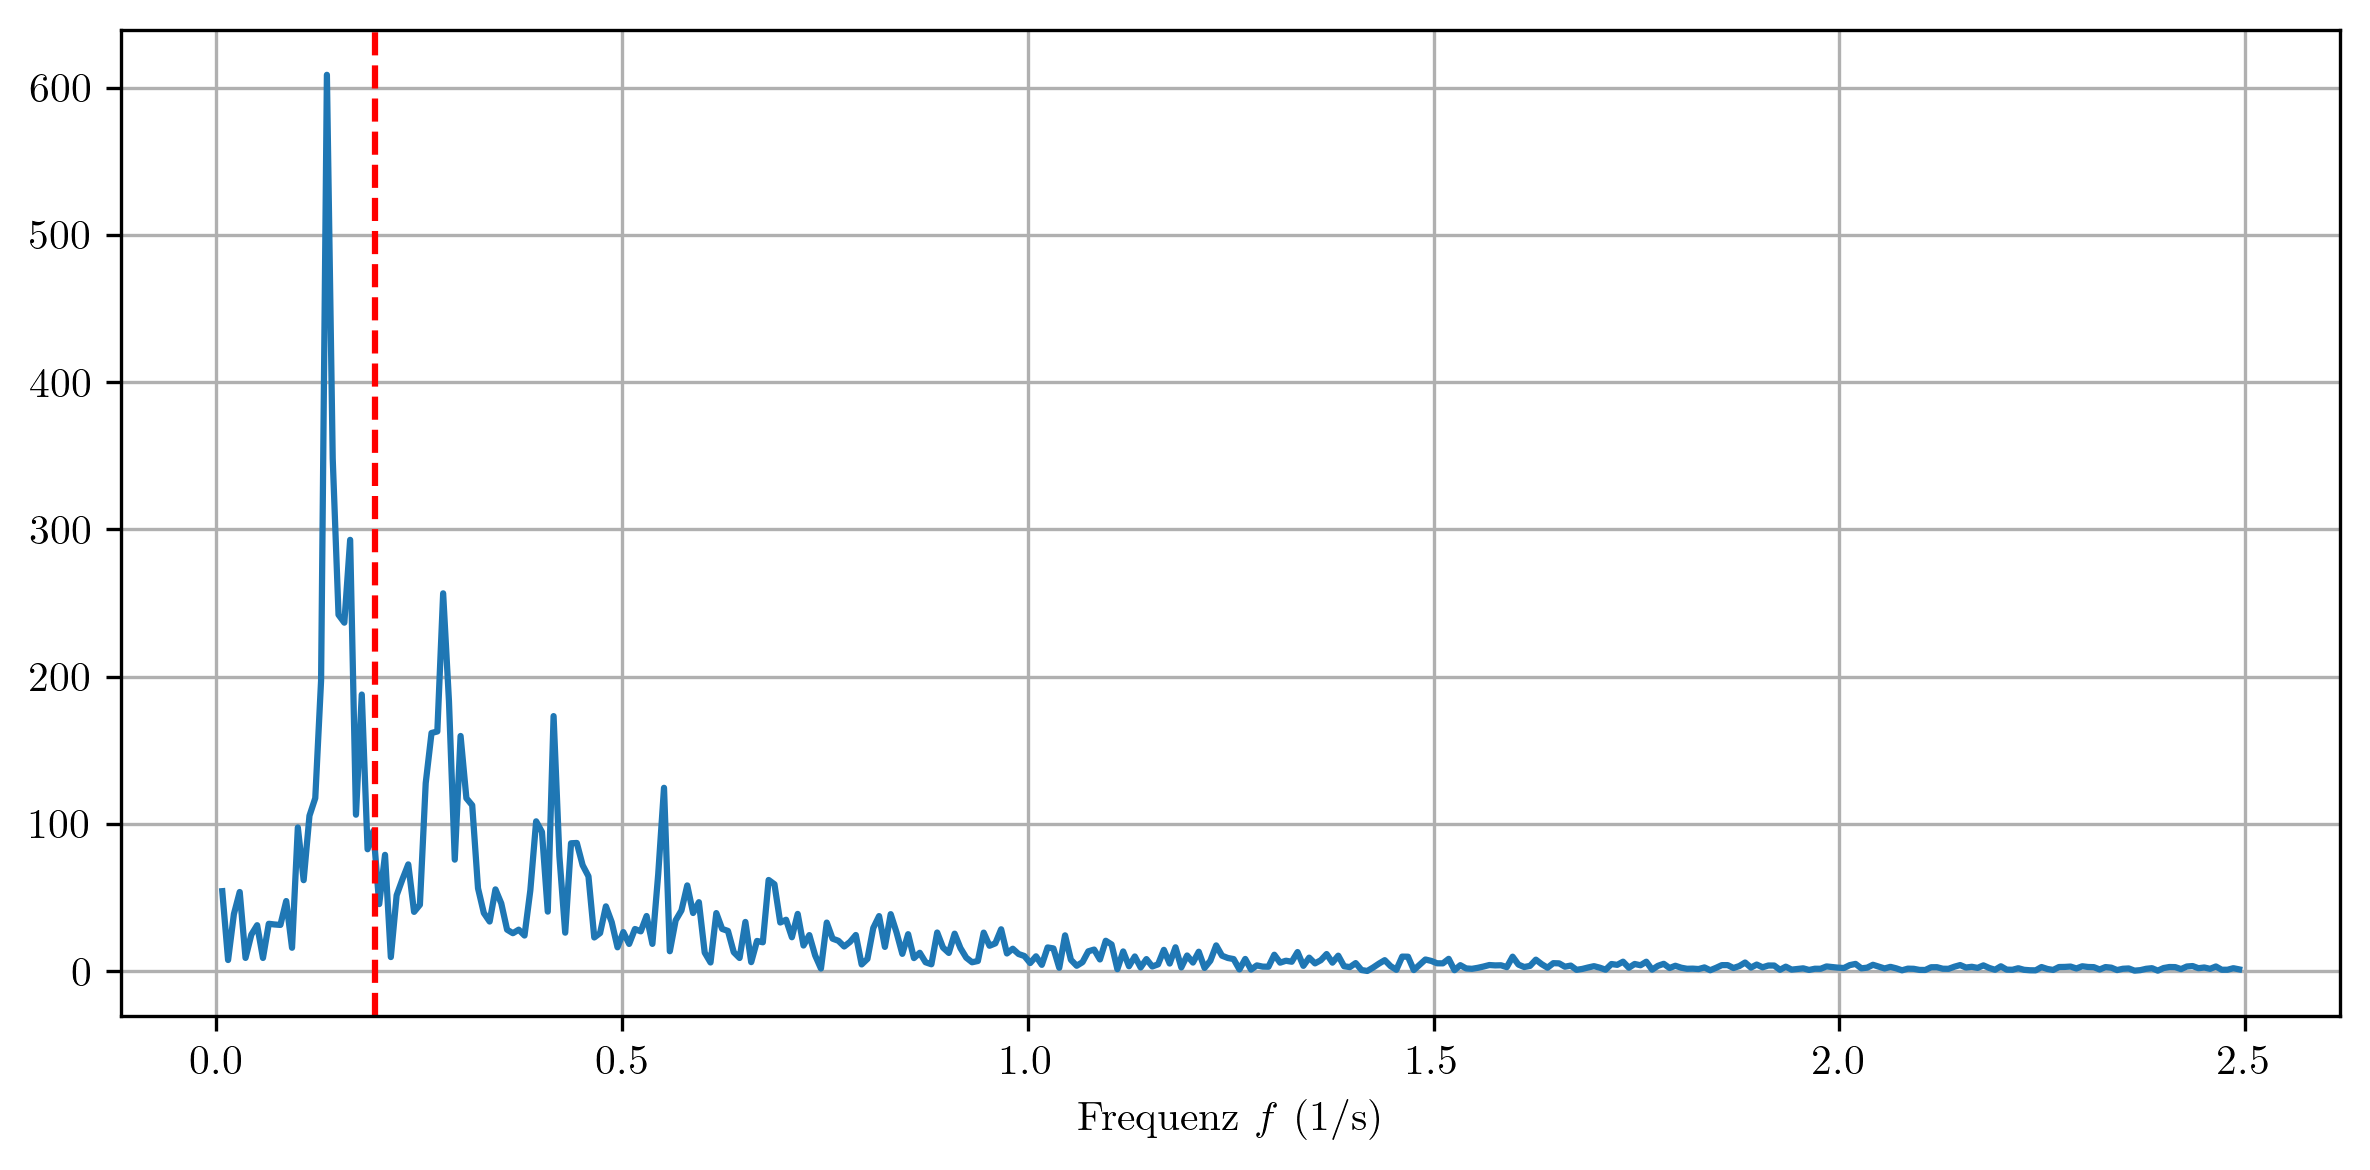
\includegraphics[width=\linewidth]{papers/reaktdiff/images/LotkaVolterra/fft_plot_latex.png}
    \caption{FFT der Animation eines Reaktionsdiffusionsmodell mit den Reaktionstermen \eqref{reaktdiff:equation:lvsys}. Die rote Linie zeigt die theoretisch dominante Frequnez von \(f = \omega / 2 \pi \approx 0.195\,\text{Hz}\). Die Abweichung kann durch generelle abweichungen in der Simulation erklärt werden}
    \label{reaktdiff:fig:lvfft}
\end{figure}
